\section{Methodology}
\label{sec:method}

\begin{figure*}[t]
\centering
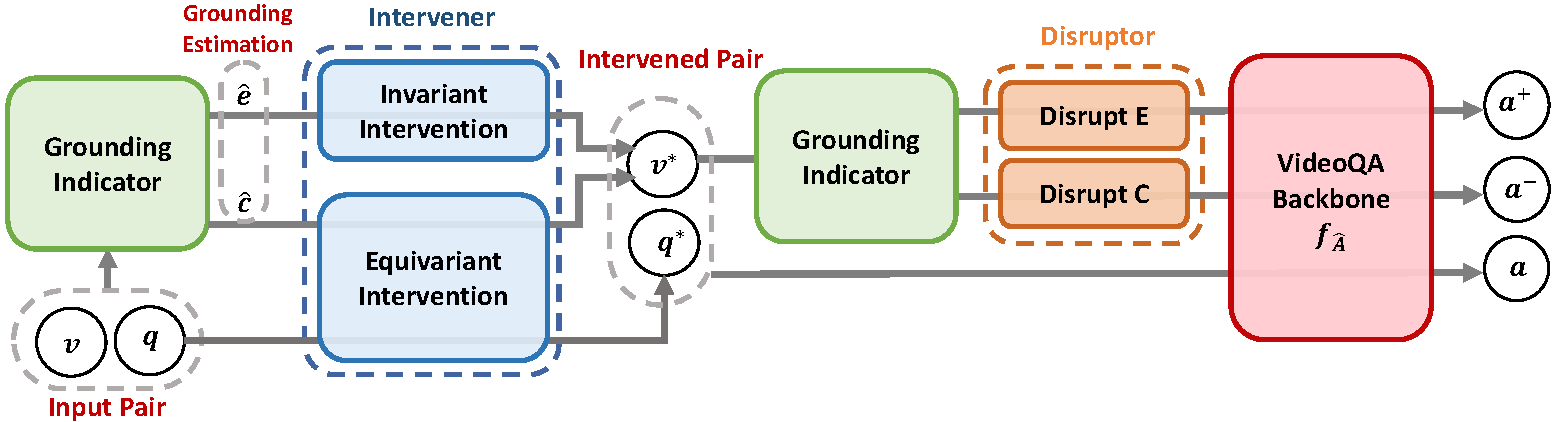
\includegraphics[width=0.95\textwidth]{fig/main.pdf}
\vspace{-14pt}
\caption{Overview of EIGV. It comprises three additional modules on top of the conventional VideoQA backbone: 1) Grounding indicator, 2) Intervener, and 3) Disrupter. First, the grounding indicator learns the estimation of causal scene $\hat{c}$ and environment $\hat{e}$. Next, two interventions are imposed on the causal and non-causal factors to compose the intervened pair $(v^*,q^*)$. Finally, based on the re-grounded result, the disruptor creates contrastive samples, which are further feed into the VideoQA backbone.}
\vspace{-5pt}
\label{fig:main}
\end{figure*}

\wx{
To ground the causal scene $C$ in the video $V$, we take a closer look at the VideoQA SCM (\ie Figure \ref{fig:scm}a), and emphasize the essential differences between $C$ and $E$.
Specifically, given the causal scene $C$ and question $Q$, the answer $A$ is determined, regardless of the variations in the environment scene $E$:}
\begin{gather}\label{equ:eq0}
      A\bot E \mid C,Q,
\end{gather}
where $\bot$ denotes the probabilistic independence. 
%

\vspace{5pt}
\noindent\textbf{Rationalization.} 
During training, the oracle grounding rationale $C$ is out of reach, while only the input $(V, Q)$ pair and training target $A$ are observed. 
Such an absence motivates VideoQA to embrace video grounding in its modeling. 
Specifically, in light of question $Q$, the estimated causal scene $\hat{C}$ is grounded from the massive $V$ to approach the oracle $C$ and then generate prediction $\hat{A}$ via $Q \rightarrow A \leftarrow C$. 
To systematize this relation, the causal-equivariance principle introduces an equivariant transformation $T_\epsilon$ to each of the parent variables (\ie $C$ and $Q$), and expects a proportionate change in the response variable (\ie $A$). On top of SCM, we formally present such notions as:
\begin{gather}
    T_\epsilon(\hat{A})=f_{\hat{A}}(T_\epsilon(\hat{C}),T_\epsilon(Q)). \label{equ:equivariance}
\end{gather}
Meanwhile, environment-invariant principle formulated Equation \eqref{equ:eq0} in the sense that imposing an invariant-transformation $T_\iota$ on the estimated environment $\hat{E}$ should not trigger variation of answer $A$: 
\begin{gather}
      \hat{A}=f_{\hat{A}}(T_\iota(\hat{E}),Q)),\label{equ:invariance}
\end{gather} 
To this end, we parameterize our learning framework, EIGV, as a combination of equivariant and invariant principles, which comprises three additional modules on top of the ERM-guided backbone: grounding indicator, intervener, and disruptor. In a nutshell, we display our EIGV framework in Figure \ref{fig:main}.


\vspace{5pt}
\noindent \textbf{Data representation.}
Following previous efforts \cite{jiang2020reasoning, DBLP:conf/acl/GuoZJ0L20}, we encode video instance $v$ as a sequence of $K$ fixed visual clips, while question instance $q$ is encoded into a similar form with a fixed length of language tokens $L$.
Then, visual and linguistic features are applied with a linear layer and an LSTM \cite{10.1162/neco.1997.9.8.1735}, respectively, to align their dimension. As a result, we acquire the output of linear layer $ \vb{v} \in \mathbb{R}^{k \times d}$ as the final video representation and the last hidden state of LSTM $\vb{q} \in \mathbb{R}^{d}$ as the holistic question representation.

% Following previous efforts [], video instance $v$ is encoded as a sequence of $K$ fixed visual clips $ \vb{v} \in \mathbb{R}^{k \times d_v}$, where $d_v$ is the visual feature dimension. Likewise, the question instance $q$ is encoded into similar form $ \vb{q} \in \mathbb{R}^{L \times d_q}$ but with a fixed length of language tokens L. Furthermore, $\vb{v}$ and $\vb{q}$ are respectively, applied with a linear layer and a LSTM [] to align their dimension, while we acquire the final hidden state of LSTM as a the holistic question representation $\vb{q} \in \mathbb{R}^{d}$.

\subsection{Grounding Indicator}
Scene partition is fundamental to the rationale discovery, whose core is to estimate the value of $C$ and $E$ via a hard split on video $V$. Given an input sample $(v,q)$, the grounding indicator aims to access the causal scene and environment scene via their estimated value $\hat{c}$ and $\hat{e}$ according to question $Q$. 
%
Concretely, we first construct two cross-modal attention modules to indicate the probability of each visual clip of being causal scene ($\vb{p}_{\hat{c}} \in\mathbb{R}^{K}$) 
and environment scene ($\vb{p}_{\hat{e}}\in\mathbb{R}^{K}$):
\begin{align}
    \vb{p}_{\hat{c}} &= \text{Softmax}(\text{FC}_{1}(\vb{v})\cdot\text{FC}_{2}(\vb{q})^\intercal),\\
    \vb{p}_{\hat{t}} &= \text{Softmax}(\text{FC}_{3}(\vb{v})\cdot\text{FC}_{4}(\vb{q})^\intercal),
\end{align}
where $\text{FC}_{1},\text{FC}_{2},\text{FC}_{3},\text{FC}_{4}$ are fully connected layers that align cross-modal representations.
%
However, gathering messages via a soft mask still makes the visual information on different clips overlap. 
As discussed in Section 3.2, guided by ERM, the conventional attention mechanism is unable to block the influence of $\hat{e}$, thus undermining the veracity of $\hat{c}$.
% As revealed by the ERM-guided method, the conventional attention is unable to block the influence of $\hat{t}$ thus undermining the veracity of $\hat{e}$. 
%
As a correction, the grounding indicator makes a discrete selection over the clip-wise attention result to generate a disjoint group of the causal scene. We leverage Gumbel-Softmax \cite{DBLP:conf/iclr/JangGP17} to manage a differentiable selection on attentive probabilities and compute the indicator vector $\vb{I}\in\mathbb{R}^{K\times 2}$ on the two attention scores  over each clip (\ie $\vb{p}_{\hat{c,i}}$, $\vb{p}_{\hat{e,i}}$, $i \in K$).  Formally, $\vb{I}$ is derived as:
\begin{gather}
    \vb{I} = \text{Gumbel-Softmax}([\vb{p}_{\hat{c}};\vb{p}_{\hat{e}}]), 
\end{gather}
where $[;]$ denote concatenation. The first and second column of $\vb{I}$ (\ie $I_{0}$ and $I_{1}$) index the attribution of $\hat{c}$ and $\hat{e}$ over k clips, respectively. 
%
To this end, we estimate $\hat{c}$ and $\hat{e}$ as follows:
\begin{gather}
    \hat{c} = I_{0}\cdot v ,\quad \hat{e} = I_{1}\cdot v, \quad \st v=\hat{c}+\hat{e} .
    % \hat{c} = \{I_{c,k}\cdot v_{k}|I_{c,k}=1\},\quad \hat{t} = \{I_{t,k}\cdot v_{k}|I_{t,k}=1\},
\end{gather}

% where binary masks $I_{0k}$ and $I_{1k}$ indicate the causal-environment attribution of the $k$-th clip.

\subsection{Intervener}
In absence of clip-level supervision, learning grounding indicators requires dedicated exploitation of the equivariance-invariance principle.
%
On this demand, we propose the intervener, which prompts the estimated rationale to the oracle by intervening $\hat{c}$ and $\hat{e}$. 
%
Figure \ref{fig:intervene} describes the functionality of $do(\cdot)$ --- the intervention operator that successively manipulated SCM over $E$ and $C$. Concretely, two intervention operations are configured to realize the equivariant and invariant transformation defined in Equations \eqref{equ:equivariance} and \eqref{equ:invariance}. 
%
% 这块儿写的不清楚。要牢记突出主线:two principle,所有的都是围绕这个实现的,只有我们反复强调这个,才能让reviewer印象深刻,然后才能从idea、implementation层面上都理解我们在干啥,并且觉得我们做的是对的。
% 这里可以分开写:

To fulfill the causal-equivariant principle, we design the E-intervention on the causal scene $\hat{c}$, which applies a linear interpolation between two data points on their causal factors --- $C$, $Q$ and $A$.  
By casting the same mixing ratio $\lambda_0\sim\text{Beta}(\alpha,\alpha)$ on all causal factors, the equivariant intervener learns to capture 
% the mainstay depicted in Figure \ref{fig:scm}c, so as to abridge 
the causal connection of $C, Q \to A$.
In particular, we attain the intervened causal scene $c^*\in \mathbb{R}^{K\times d}$, question $q^*\in \mathbb{R}^{d}$ and answer $a^*\in \mathbb{R}$ as follow:
\begin{gather}
    c^*=\lambda_0 \cdot \hat{c}+(1-\lambda_0) \cdot \hat{c}',\\
    q^*=\lambda_0 \cdot q+(1-\lambda_0) \cdot q',\\
    a^*=\lambda_0 \cdot a+(1-\lambda_0) \cdot a',
\end{gather}
where $\hat{c}'$, $q'$ and $a'$ are causal factors from a second sample.

To achieve the environment-invariant principle, we devise the I-intervention that adopts a similar mixing strategy to the environment scene $\hat{e}$. 
%
Notably, by drawing the mixing ratios $\lambda_1$ from a second distribution that is distinct from the equivariant one (\ie $\lambda_1\sim\text{U}(0,1)$), the invariant intervention learns to rule out the influence of environment scene on the answer, which essentially refines the ERM-guided scheme at our will. 
Formally, we arrive the intervened environment scene $e^*$ by:
\begin{gather}
    e^*=\lambda_1 \cdot \hat{e}+(1-\lambda_1) \cdot \hat{e}',
\end{gather}
where $\hat{e}'$ is the estimated environment scene of a second sample.

In practice, the equvariant and invariant intervention operations are performed in parallel on different parts of $v$, and the intervened video $v^* \in \mathbb{R}^{K\times d}$ is composed of $do(C=c^*)$ and $do(E=e^*)$:
% in a cascade manner:
\begin{gather}
    v^*=c^*+e^*.
\end{gather}

% where $\hat{c}'$ and $\hat{e}'$ are estimate causal and environment scene of dummy  sample ($v',q',a'$).  It's worth noticing that, the mixing ratios $\lambda_0$ and $\lambda_1$ for equivariant and invarinat intervention are drawn from two different distribution, $\lambda_0\sim\text{Beta}(\alpha,\alpha)$ and $\lambda_1\sim\text{U}(0,1)$.
% %
% To complete the reasoning logic, we also apply the equivariant intervention on other causal factors---$Q$ and $A$ to generate intervened question $q^*$ and answer target $a^*$:
% \begin{gather}
%     q^*=\lambda_0 \cdot \hat{q}+(1-\lambda_0) \cdot q',\\
%     a^*=\lambda_1 \cdot \hat{a}+(1-\lambda_1) \cdot a',
% \end{gather}
% Noticably, we cast the same equivariant mixing ratio $\lambda_0$ for $do(Q)$ and $do(A)$ to abridge the the causal connection of $C,Q \to A$. 

% 
\subsection{Disruptor}
% In state-of-the-art self-supervised learning (SSL) pre-training produces semantically good representations by encouraging them to be invariant under meaningful transformations prescribed from human knowledge. 

To fully exploit the privilege of the proposed principles, we employ contrastive learning as an auxiliary objective to establish a good representation that maintains the desired properties of $\hat{c}$ and $\hat{e}$. 
% discribe in  to the counterfactual substitution on $C$($E$). 
Specifically, we first compose a memory bank $\pi$ as a collection of visual clips from other training videos. Then, we apply the grounding indicator a second time on top of the intervened variables, where the re-grounded causal and environment scene are manipulated to set up the contrastive twins as follows:
\begin{itemize}[leftmargin=*]
% 介绍清楚,为啥相对于anchor而言就是positive的
\item In light of the environment-invariance principle, positive video is developed in the sense that changing the environment scene will not provoke disagreement in answer semantics.  Thus, the disruptor synthesizes a positive video $v^+$ by disrupting the $v^*$ on its environment part --- that is, replacing the environment scene with a random stratification sampled from the memory bank.\footnote{Note that the environment substitutes will not involve the question-relevant scenes, to avoid creating additional paths from $E$ to $A$.}  
% 介绍清楚,为啥相对于anchor而言是negaitve的
\item Built upon the causal-equivariance principle, the negative counterpart $v^-$ is created by a similar disruption but on the causal scene of $v^*$, where substitution on the question-critical causal part should raise inconsistency in answer space.
% \footnote{substitution of causal scene substitutes will not involve the question-relevant scenes, to avoid creating additional paths from $E$ to $A$.} 
%
Apart from the visual negatives, the disruptor also creates linguistic alternatives to enhance the distinctiveness of the vision-language alignment. Specifically, it disrupts the combination of the intervened input ($v^*, q^*$) and pairs the video with random sample question $q_r$ to create a second view of negative samples ($v^*, q_r$).
\end{itemize}
To this end, we attain the answer representation of anchor $\vb{a}$ and its contrastive counterparts $\vb{a}^+, \vb{a}^-$ by feeding the paired positive and negative samples to backbone VideoQA model $f_{\hat{A}}$: 
\begin{gather}
    \vb{a}=f_{\hat{A}}(v^*,q^*),\\
    \vb{a}^+=f_{\hat{A}}(v^+,q^*),\\
    \vb{a}^-=f_{\hat{A}}([(v^-,q^*);\,(v^*,q_r)]),
\end{gather}
where $[;]$ denotes concatenation.

Notably, EIGV is designed to be model-agnostic, which aims to promote any VideoQA backbone built on frame-level visual inputs.
%
% Since the architecture modification is beyond our intention, we verify the effectiveness of our design by marrying EIGV to SoTA VideoQA models. 




\subsection{Optimization}
By far, we set up the intervened vision-language instance ($v^*,q^*$) for a pair of input ($v,q$), and further constitute its contrastive counterparts based on the estimated grounding result. 
To steer the learning process away from the conventional ERM pitfall, we establish two learning objectives on top of their output $a, a^+, a^-$:

\begin{itemize}[leftmargin=*]
    \vspace{5pt}
    \item \noindent \textbf{Contrastive loss.} To reflect the invariant property of the environment scene while maintaining the distinctiveness of the causal scene, we borrow the definition of InfoNCE \cite{DBLP:journals/corr/abs-1807-03748}, and construct the contrastive objective as follows:
    \begin{gather}
        \mathcal{L}_{CL}=-log(\frac{\text{exp}{(a^\top a^+)}}{\text{exp}{(a^\top a^+)}\,+\sum_{n}^{N}\text{exp}{(a^\top a_n^-)}}),
    \end{gather}
    where $N$ is the number of negative samples, \lyc{$a_n^-$ denotes negative anwer generated by one of  negative samples.} 
    
    \vspace{5pt}
    \item \noindent \textbf{ERM loss.} 
    Estimating the rationale requires a robust causal connection from $V,Q$ to $A$. Thus, we imposed an entropy-based risk function \lyc{$\text{XE}(\cdot)$} on $(v^*,q^*)$ to approach the intervened answer $a^*$:
    \begin{gather}
        \mathcal{L}_{ERM}=\text{XE}(f_{\hat{A}}(v^*,q^*), a^*),
    \end{gather}
\end{itemize}

As a result, the overall training objective of EIGV is the aggregation of the forgoing risks:
\begin{gather}
   \mathcal{L}_{\text{EIGV}} = \mathbb{E}_{(v,q,a)\in\mathcal{O}}\mathcal{L}_{ERM} + \beta\mathcal{L}_{CL},
\end{gather}
where $\mathcal{O}$ is the set of training instances $(v,q)$ alongside their ground-truth answer $a$; $\beta$ is the hyper-parameter that balances the strength of contrastive learning. The joint optimization disentangles the mischief of environment scene, thus fulfilling the desired interpretation by locating the causal pattern. During inference, EIGV generates the predication $\hat{a}$ without the intervener and disruptor involved, and gives the interpretation $\hat{c}$ as the partition result of the grounding indicator.

% Specifically, by minizing the  the similarity between en-
% coded representations of the same video at two
% different speeds as well as minimize the sim-
% ilarity between different videos played at dif-
% ferent speeds, leveraging the fact that changing
% video speed does not change an action on both
% domains.


% an oracle interpretation $C$ should reflect the semantic variance of different $Q$ and trigger the corresponding change in $A$,

% video input tend to contain multiple visual scene, but only the question-relevant part contributes to the prediction while the rest is inconsequential to the reasoning logic.


\begin{figure}[t]
\centering
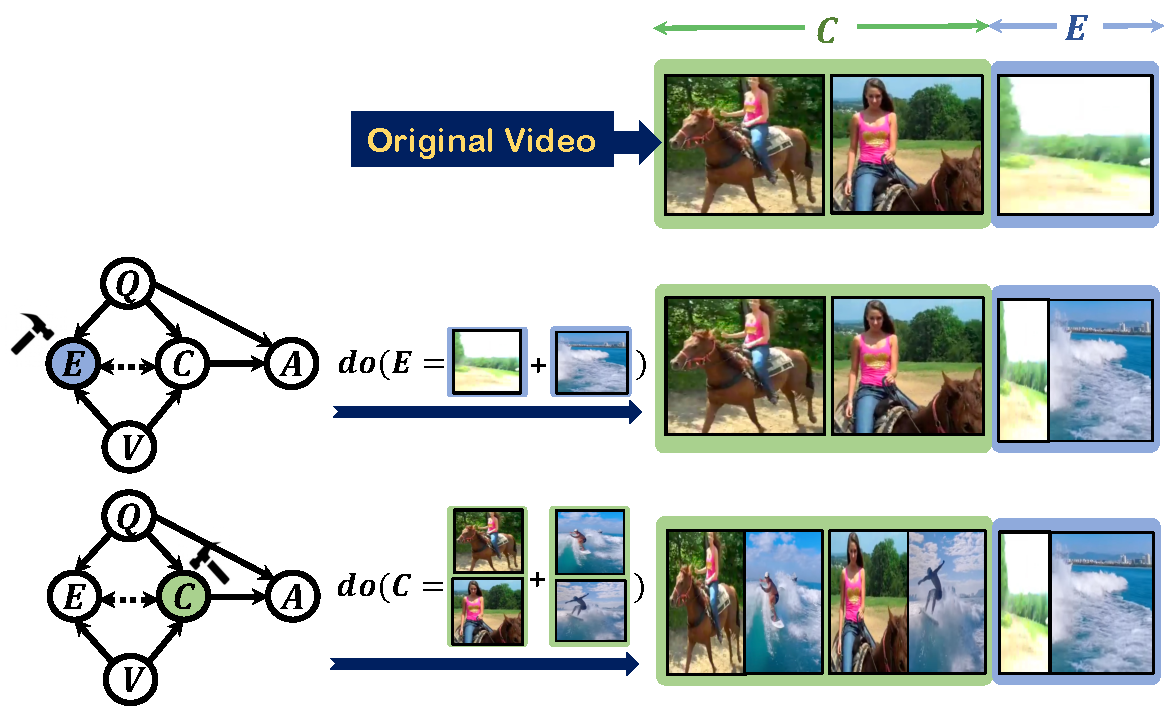
\includegraphics[scale=0.43]{fig/intervene.pdf}
\caption{We illustrate the invariant and equivariant interventions in the second and third rows, respectively. The effects on $Q$ and $A$ are omitted for illustration purposes.}
\vspace{-5pt}
\label{fig:intervene}
\end{figure}